\documentclass[conference]{IEEEtran}
% \IEEEoverridecommandlockouts
% % The preceding line is only needed to identify funding in the first footnote. If that is unneeded, please comment it out.
\usepackage{cite}
\usepackage{amsmath,amssymb,amsfonts}
\usepackage{algorithmic}
\usepackage{graphicx}
\usepackage{textcomp}
\usepackage{xcolor}
\def\BibTeX{{\rm B\kern-.05em{\sc i\kern-.025em b}\kern-.08em
    T\kern-.1667em\lower.7ex\hbox{E}\kern-.125emX}}
\pagenumbering{roman}

\begin{document}

\title{Addictive Design Strategies in Software Development\\
\large Understanding its Form and Impact in the context of Social-Media Applications}

\author{

\IEEEauthorblockN{Saurav Kumar, Samarth Mehta, Lax Kyada, Ashawini Chudaman}
\IEEEauthorblockA{\textit{Department of Computer Science} \\
\textit{Virginia Tech, Blacksburg, VA}}
}

\maketitle

\begin{abstract}
Lorem ipsum dolor sit amet, consectetur adipiscing elit, sed do eiusmod tempor incididunt ut labore et dolore magna aliqua. Ut enim ad minim veniam, quis nostrud exercitation ullamco laboris nisi ut aliquip ex ea commodo consequat. Duis aute irure dolor in reprehenderit in voluptate velit esse cillum dolore eu fugiat nulla pariatur. Excepteur sint occaecat cupidatat non proident, sunt in culpa qui officia deserunt mollit anim id est laborum.
\end{abstract}

\begin{IEEEkeywords}
put some keywords
\end{IEEEkeywords}

\section{Introduction}
Until some time ago, the concept of ethics in software engineering was a new one. In a more traditional sense, it didn't make a lot of sense to question the ethics of software engineering techniques as applications back then did not have the mass appeal and reach, as applications today do. However, with changing times, we are now encountering software applications at every stage of our day-to-day lives. This increased demand for services has been met with changing business ideals from tech companies, which has led to several instances of scientists, philosophers and even common consumers questioning the ethics of  certain software engineering practices. Traditionally, for most businesses the user was the target commodity. This system was called an {\it ad-based} economy model and it has been around for centuries \cite{wu2016}. This has changed however. Today, businesses' target commodity is a user's attention. Businesses do not charge consumers directly for the services, but instead sell this target commodity to their customers (e.g., advertisers, other businesses, etc) \cite{williams2018}. Such a system is called an {\it attention-based} economy model and, the richest and most influential companies to come out of this model are social media companies \cite{pwc2018}.

We have seen that a lot of attention is being paid towards understanding the impact of social media, especially in the ways that it can be used to cause distress or harm (e.g., to bully people online \cite{campbell2005}, to incite certain groups of people towards violence \cite{huey2015}, to polarize and alienate people from society \cite{sunstein2017}, etc.). While these issues are very important too, they are based on how these powerful applications are being misused by people, whether it's a person bullying another person or a politician inciting sectarian disharmony. This article, however, attempts to peek behind the veil of the fundamentals of this {\it attention-based} economy model and focuses on the {\it addictive design} strategies being used by businesses to increase a customer's engagement and retention.

\subsection{Our Addiction to Internet}
According to a recent study \cite{uswitch2021}, an average citizen of the United Kingdom uses internet for up to 6.4 hours every day and watches 1350 hours of TV every year, on average. On the other side of the ocean, Americans aren't doing better either. An average American citizen, spends 325 hours per year and 297 hours per year on Facebook and Instagram respectively. Studies are showing that kids of the age group of 5 to 16 years are spending up to 9 hours a day on social media platforms. 

Despite the technological leaps that Internet has enabled us to take, scientists, philosophers and doctors have been trying to caution us about the numerous perils of internet addiction since a long time \cite{th1996, gr1998}. Excessive usage of smartphones have been known to cause detrimental effects on our mental health \cite{sc2018}, such as loss of productivity \cite{duke2017}, lowering a person's overall well-being \cite{twenge2018}, brain-drain \cite{ward2017}, etc. A form of Internet Use Disorder (IUD), called the {\it Internet Gaming Disorder} has now been recognized \cite{pontes19} by the Diagnostic and Statistical Manual of Mental Disorders (DSM-5), which is issued by the American Psychiatric Association (APA). This leads us to a disheartening conclusion that internet and social-media addiction is a global problem which transcends socio-economic barriers and affects each one of us equally.

\subsection{Peeking behind the Veil}
A lot of people think that internet, in general, and smartphones, in particular, are the major culprits behind IUD. However, upon closer inspection, we find that its not the case and they are not the real culprits \cite{sha2019}. In fact, we need to instead look at the applications that are running over the internet, on our phones and TVs \cite{alter2017}. While a lot of studies have focused on different IUDs, very few have tried to focus on the addictive features of these applications and what characteristics make them addictive \cite{king11, alu18}.
In the following sections, we are going to investigate various features of popular social-media applications that make them potentially addictive.


\section{Related Work}
The mechanisms using which business have turned their software addictive have changed over time. We, however, find that certain mechanisms have been constantly employed to entrap a user's attention:

\paragraph{Intermittent Variable Rewards} It has been noted in past works \cite{wu2016} that “the most effective way of maintaining a behavior is not with a consistent, predictable reward, but rather with what is termed ‘variable reinforcement’— that is, rewards that vary in their frequency or magnitude”. Several applications employ the "pull-to-refresh" feature which mimics a slot machine (an alternative term for intermittent variable rewards is the {\it slot machine} effect \cite{wu2016, gr2018})

\paragraph{Desire for Social Validation} Social media applications have increasingly become platforms for seeking social validation from our family, friends, peers and even strangers. Features such as the 'Like' button, 'snap-streaks' etc. are known to put immense pressure on users to maintain a standard which is socially acceptable \cite{bosker2016, alter2017}.

\paragraph{Infinite Scrolling} Before the advent of big social media companies, life was comparatively simpler. When a user would reach the end of a web-page, that would mark the end of content. It would now be up to the user, to navigate to a different web-page or web-site to consume further information or take a rest and bow-out. Nowadays, we see infinite scroll almost everywhere; the information available to us for consumption is infinite \cite{williams2018, harris2019}.\\\\
The aforementioned works shed a lot of light on the ethically ambiguous features of social media platforms. In our opinion, there are several other mechanisms too that are being employed by social media companies that are directly contributing towards increasing application addiction. For example, when trying to access Twitter, we often land at the blue loading screen. Now this may seem to be an effect of internet issues or faulty hardware, but researchers think that it is yet another way of capturing user's attention \cite{morgan2017}. In the following sections, we attempt to identify addictive mechanisms that are being employed by popular social media platforms.

\section{Methodology}
In this section, we have explained the strategies we have used to investigate all research question. Fig 1 provides an overview of
steps taken to reach towards the conclusion. 

\begin{figure}[htbp]
\centerline{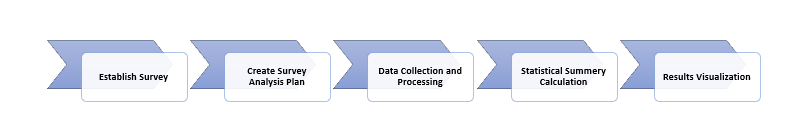
\includegraphics[width=0.5\textwidth]{Capture1.PNG}}
\caption{Methodology Steps}
\label{fig}
\end{figure}


\subsection{Initial Investigation}

To gauge the viability of our project, we have examined the trending popularity of relevant search terms using the Google Trend.

\begin{figure}[htbp]
\centerline{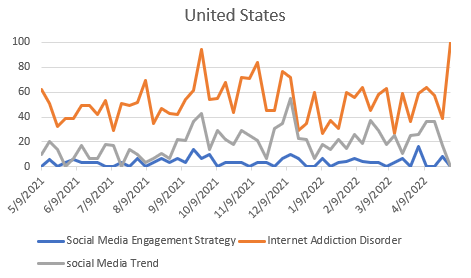
\includegraphics[width=0.4\textwidth]{US Graph.PNG}}
\caption{United States Analytic}
\label{fig}
\end{figure}

\begin{figure}[htbp]
\centerline{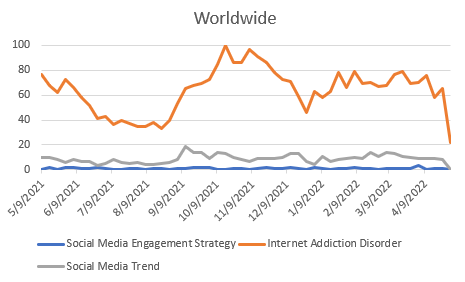
\includegraphics[width=0.4\textwidth]{Worldwide Analysis Graph.PNG}}
\caption{Worldwide Analytic}
\label{fig}
\end{figure}

Our first search trend involves the popularity of the following terms: "Social Media Engagement Strategy","Internet Addiction Disorder",and "social Media Trend", among others.Figures 1 and 2 show the relative interests of those terms, respectively, within the United States and
worldwide. The y-axis is scaled on a percentage basis such that the maximum value corresponds with 100 percent.

In the google trend analysis over the years 2021 and 2022, clearly shows increasing social media trends including short-form videos, graphics in communication, live-stream shopping, social audio strategy, along with increasing social media marking has raised its popularity worldwide. The rising investment of brands has set high grounds for capturing the customers attention.Recent surveys on increasing implementation of the social media engagement strategies categorise it as one of the major factors rising the internet addiction disorder across the united states and worldwide.During the investigation, growing popularity of the social media applications, along with multiple gaming and e-commerce applications found contributing in increasing social stress across the globe.        

Social media applications started garnering attention around year 2000. The launch of first social media application in 1997 introduced the term "social media interaction' which then witnessed huge attention specially after the launch of Facebook in 2004. After the great response to Facebook,'the social media platform', multiple other companies like Twitter, YouTube, along with other competitor companies launched their independent social media platform with different approaches implemented to achieve social interaction. Over the time, with increased exposure to the internet the social media applications and other software applications like e-commerce, gaming etc, witnessed huge traction. 


\begin{figure}[htbp]
\centerline{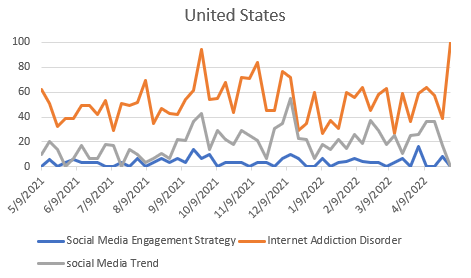
\includegraphics[width=0.4\textwidth]{US Graph.PNG}}
\caption{United States Analytic}
\label{fig}
\end{figure}

\begin{figure}[htbp]
\centerline{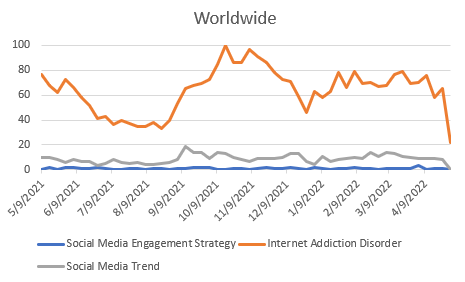
\includegraphics[width=0.4\textwidth]{Worldwide Analysis Graph.PNG}}
\caption{Worldwide Analytic}
\label{fig}
\end{figure}

\subsection{Data Collection Method}

To further explore our research topic, we collected data by conducting an online survey with questions asking respondents about their opinions and usage of the social media platforms and gaming applications. The survey, created using Google Form comprised of twenty two questions. To get a sense of the respondent demographics we included questions about topics such as participant's background in computer science or information technology, frequency of participant's interaction with online applications, along with participants' preferences or opinions for the given scenarios presenting the different ideologies useful for the study of comprehending the addictive design patterns in software development.

We believe we cultivated enough certainty for the questions about addictive design strategies in the software development to be answered honestly. Our survey offers coverage to all the aspects required for analysis of our research topic. The questions asked during the survey did not consist questions asking for personally identifiable information. In the survey, we briefly described the intentions to offer participants a quick idea about the survey topic. To make this unbiased and not discriminatory, we emphasized in our survey instructions that respondents would remain anonymous.

We have partitioned the research process across different categories useful to achieve end results and designed the survey questionnaire addressing the problems descried under specific categories. After framing survey questionnaire we distributed a shortened URL to our survey through a variety of means. We posted links to the survey on university forum, and also shared it within multiple social groups.Besides this, we circulated the survey via secondary connections.Friends and family offered to connect people they knew to encourage further participation.

In total, we managed with gather 35 survey responses from university students. Our data shows that we received submissions from participants from both technical as well as non-technical backgrounds. We believe that the different technical community belongings of our project members majorly worked to our advantage. All members of the project group majorly comes for India so we all manged to collect some responses from both of the countries - India as well as the United States.  

The following is the link to our survey: https://docs.google.com/forms/d/e/1FAIpQLSfHpX924y-A1JAzS2g9E4RwuGPXfZpE59xIJORoAFJ4oK9VxQ/viewform 

\subsection{Sampling Method}

In this subsection, we will talk about the demographics of
our survey respondents including participants' technical experience or expertise in the domain of computer science along with their frequency of using online platforms on day-to-day basis.

\begin{figure}[htbp]
\centerline{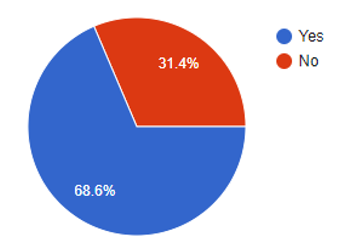
\includegraphics[width=0.45\textwidth]{Technical_Expertised Entries.PNG}}
\caption{Technical background responses analysis}
\label{fig}
\end{figure}

\begin{figure}[htbp]
\centerline{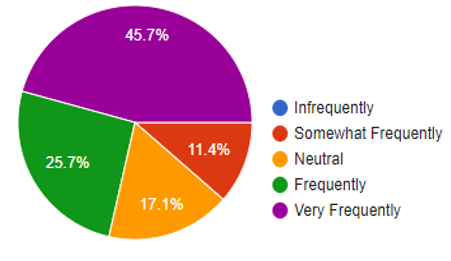
\includegraphics[width=0.48\textwidth]{Usage Frequency.PNG}}
\caption{Online platform usage frequency analysis}
\label{fig}
\end{figure}
Firstly, figure 6  represents the distribution of data against the data entries received from the participates from technical as well as non-technical backgrounds. From the graphical representation of the data it is easy to visualize and make analysis that group of participants from technical experience or expertise in the domain of computer science forms the majority class. So, data received from the survey was not highly biased towards the one particular class of survey participants. During the data analysis and data sampling we have intentionally rejected the sampling data based on race, gender or community. This aspect of data sampling making the survey analysis more ethical and obeys all ethical standards of research. 

In figure 6, the data has been sampled across five classes based on the survey responses on frequency of using online platforms on day-to-day basis. The obtained information visualization presents  majority class of survey participants who very frequently uses online platforms in their daily life. From the total data, 46 percentage of data has been captured by 'very frequently usage class' followed by the 'frequently usage class' encompassing 26 percentage of overall entries. Rest of the data entries are highly dedicated to the class of participates who are neutral,less or somewhat frequently use online applications. Our overall analysis after the prepossessing of the data shows that people participated in this survey hold technical experience or expertise in the domain of computer science and they frequently employ online application in their daily routine. Having this analysis, such participants presents the best survey responses with the great understanding on software development and addictive software design strategies.

\subsection{Data Analysis}

After successfully conducting survey and collecting \& prepossessing data we have manually evaluated our data to achieve results across the range of attributes. For data analysis we considered same categories previously used while designing the survey questions.The list of these categories includes Endless scrolling/streaming, Endowment effect/mere-exposure effect, Social pressure, Show users of an app what they like, Social comparison and social reward, and Zeĭgarnik effect/ovsiankina effect. The compete data analysis against different attributes was them made considering the inputs of each attribute dedicated to the each research process category. For this project, the list of categories can also considered as psychological mechanisms built-in social media/messenger applications and/or freemium games.

We preferred manual data analysis considering the nature of the data obtained. During analysis, different attributes (achieved by extracting the necessary knowledge from the survey questions) considered in subsets to frame research results. For instance, participants with technical experience or expertise in the domain of computer sciences and frequently use online platforms are considered better candidates for questions involving developers' opinions. All other entries are more likely considered for questions having more emphasis on understanding the participants' opinion as a user of online applications consisting addictive design strategy. Overall, analysing different attributes in combinations helped us achieve accurate research results.   

For statistics we primarily used frequency and percentage since they provide a straightforward summary statistic that can be easily understood by multiple audiences. These are most often used for multiple-choice and rating scale survey response options. Overall, techniques used for deriving information from the raw data has helped us produce research project results and offer information visualization. 

\section{Results}
We have categorized our questionnaire into 6 major categories and in the following sub-sections, we show the results of our analysis, along with their interpretations.

\begin{figure}[htbp]
\centerline{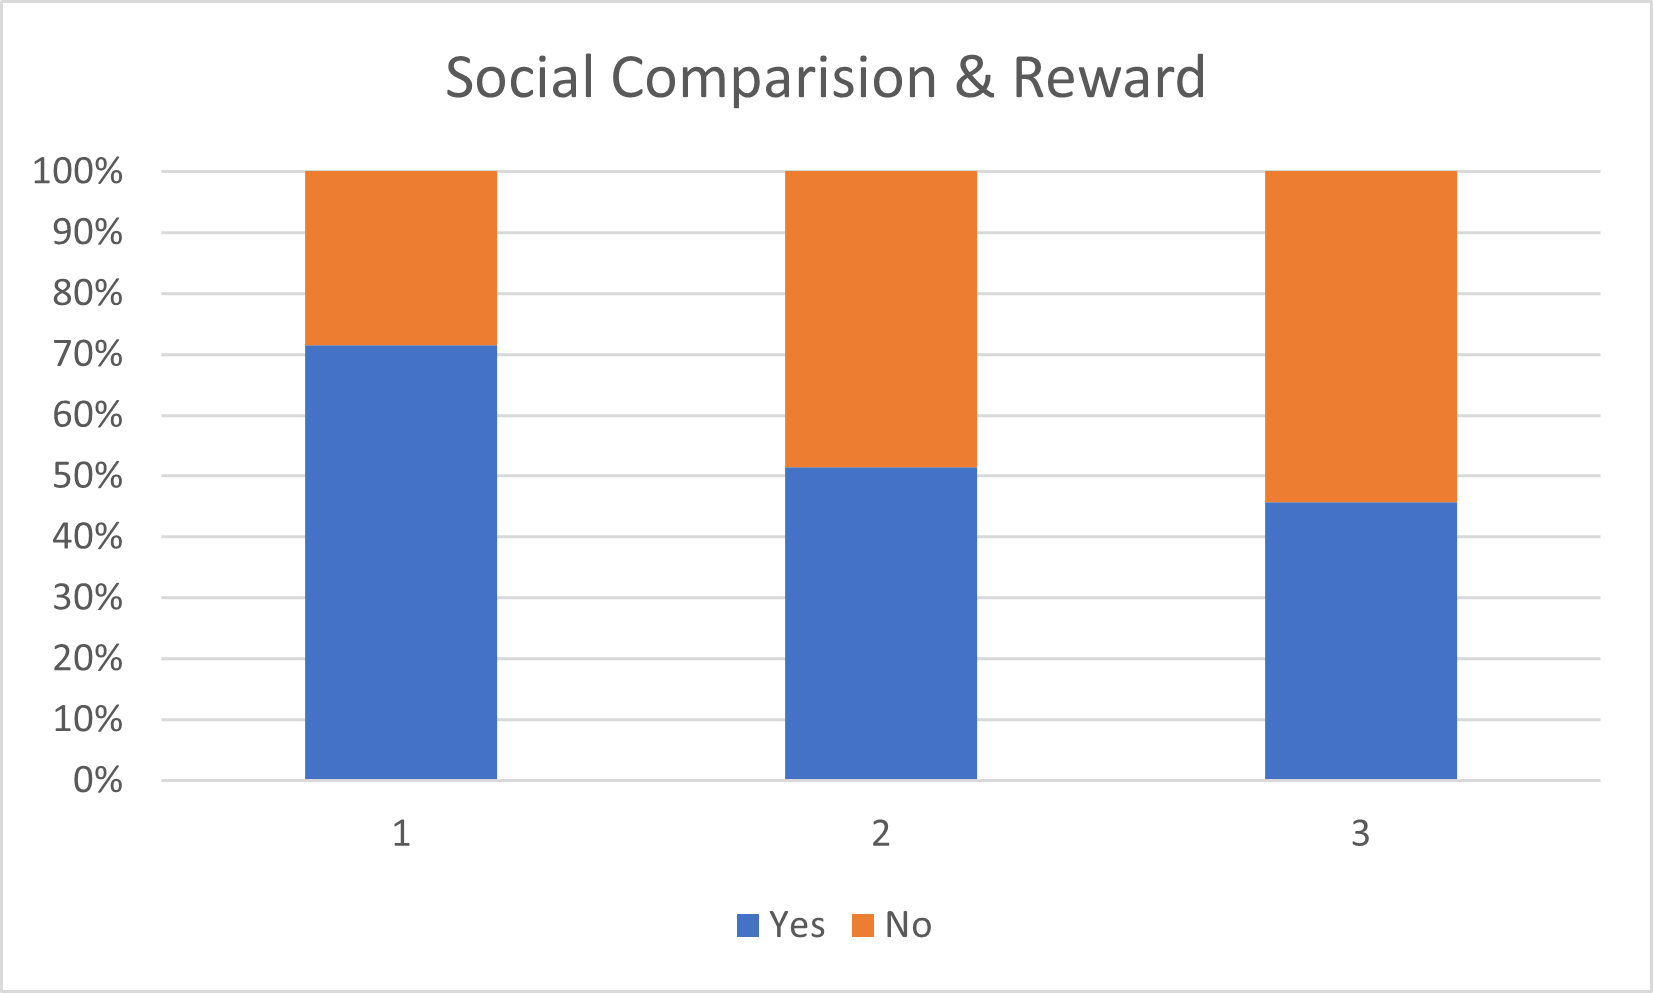
\includegraphics[width=0.5\textwidth]{SR.png}}
\caption{Distribution of responses to questions based on social comparison and reward mechanism.}
\label{sr}
\end{figure}

\subsection{Social Comparison and Reward} 
\textbf{Objective:} Most of the social media platforms host some sort of social reward feature which could be present in various forms, ranging from 'Like' to 'Upvote'. We asked 3 questions from this section in the survey.

The first question [\textit{As a user, do you think app users feel upset, angry or resentful when their social media posts do not garner enough likes, retweets, shares or similar?}] is aimed towards understanding impact of social-media addiction on human emotion. The second question [\textit{Few social media apps have recently started hiding the number of likes and dislikes that a user's post gets. Do you think this would help in combating the problems being caused by such a reward-based system?}] focuses on gauging the trust that  consumers have on social-media platforms in terms of them identifying and fixing issues being caused by addictive designs. The final question [\textit{If you were given the chance to create your own app, would you use a similar rewarding system [e.g., Likes, Shares, etc.] as is being used by other major social media apps?}] focuses on a human's perception of the necessity for addictive design.\\

\textbf{Observations:} The responses received for this set of questions were recorded in a CSV file and the initial values of \textit{YES} and \textit{NO} were mapped to 1 and 0, respectively. Based on this dataset, the distribution of responses was plotted in Fig.~\ref{sr}. 

We observed that approximately 71\% of the respondents relate to the fact that addictive usage of social media's social reward features illicit strong emotional response in users. While majority of the respondents agree that social-media triggers strong emotional response, only 51\% believe that removing social reward mechanism from applications will have any impact on reducing addiction to these platform. Interestingly, this indifference to presence of a social reward feature is also evident by the responses to the third question, wherein only 54\% of the surveyed group would \textbf{NOT} want to use a similar reward system if they were to ever create their own social media platform.

\begin{figure}[htbp]
\centerline{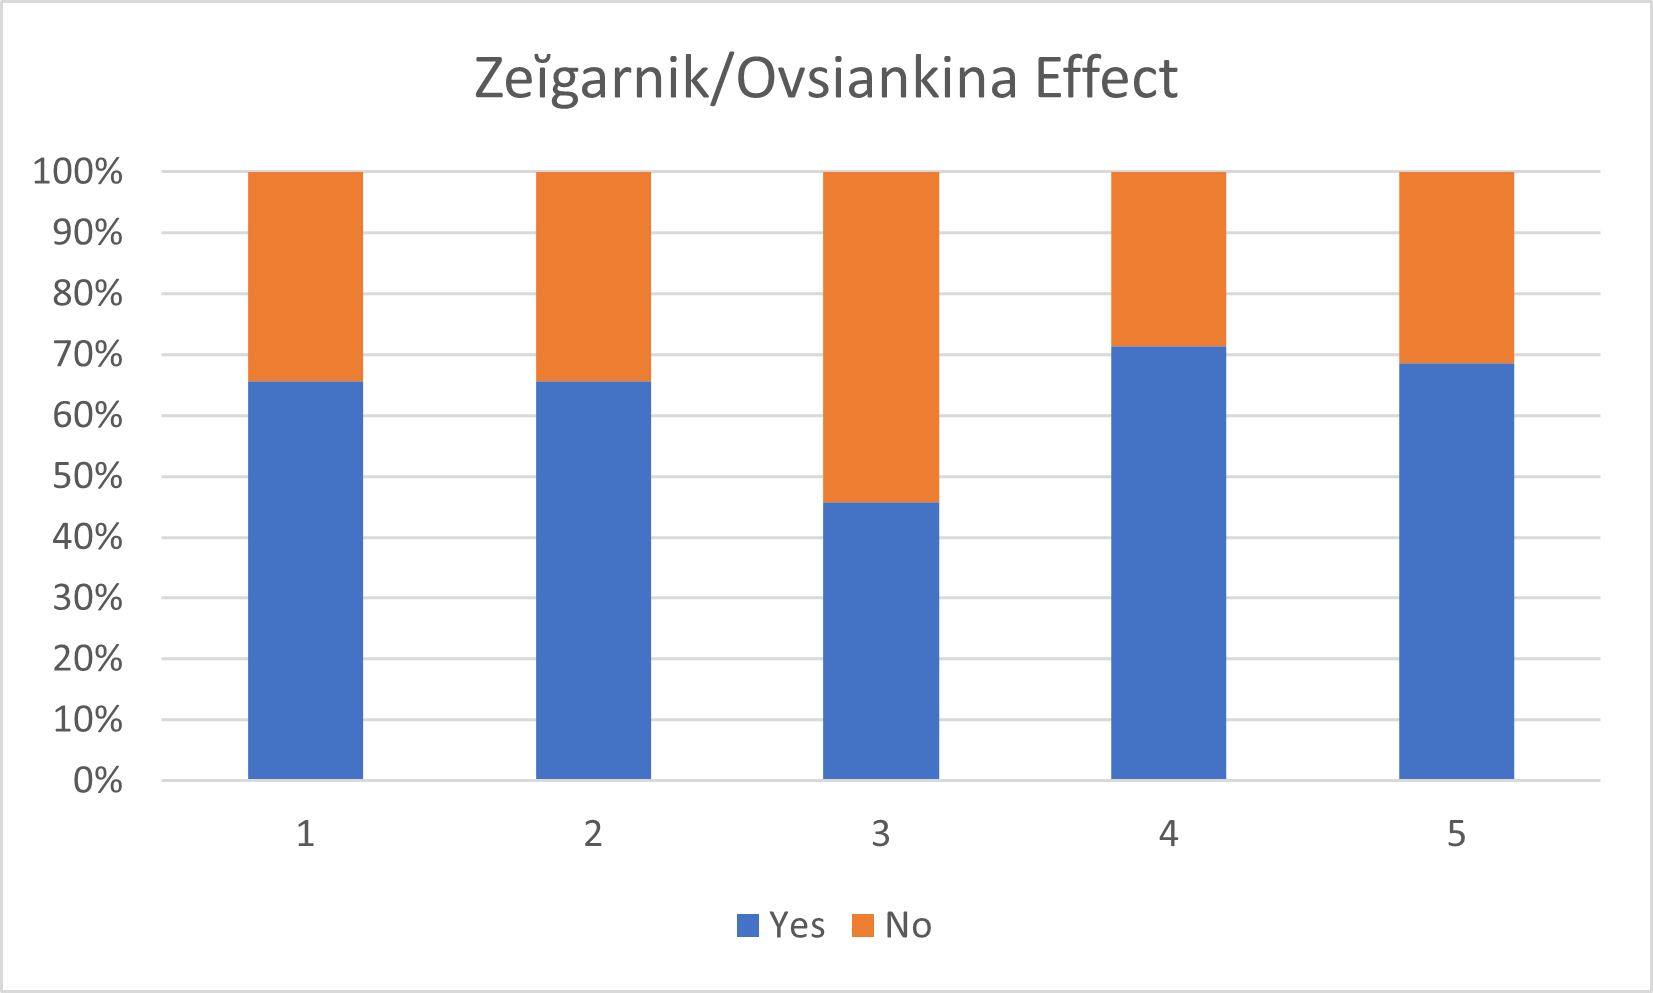
\includegraphics[width=0.5\textwidth]{ovi1.png}}
\caption{Distribution of responses to questions based on Zeĭgarnik/Ovsiankina effect}
\label{ovi1}
\end{figure}

\begin{figure}[htbp]
\centerline{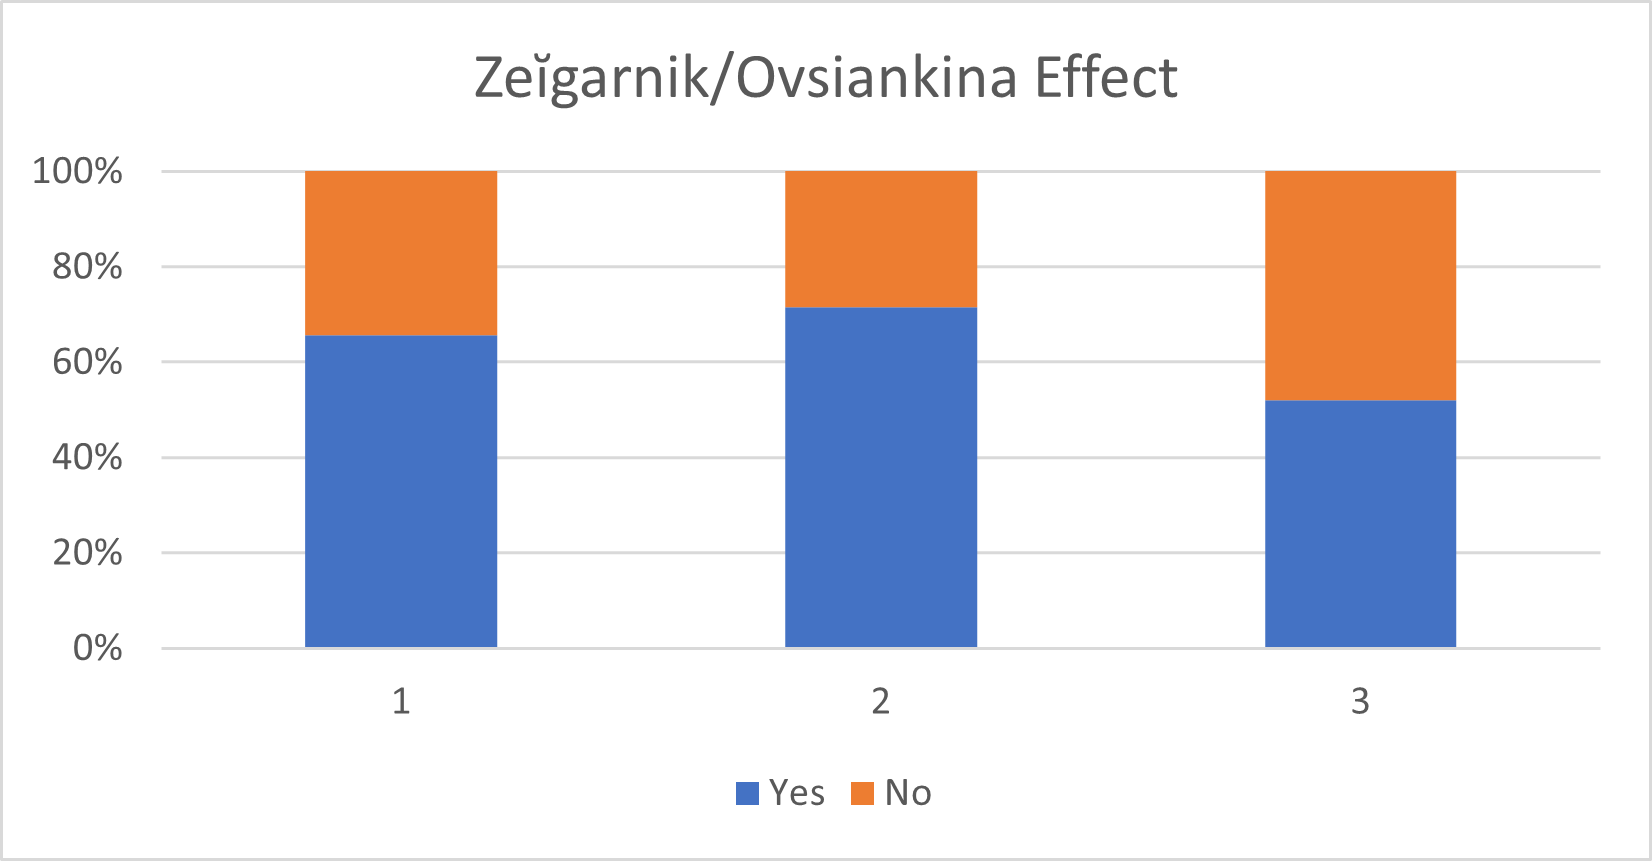
\includegraphics[width=0.5\textwidth]{ovi2.png}}
\caption{Distribution of aggregated responses based on question categories}
\label{ovi2}
\end{figure}

\subsection{Zeĭgarnik/Ovsiankina effect}
\textbf{Objective:} In a classic set of experiments \cite{zie1927, kina1928}, scientists observed that when individuals were interrupted in a task, it was seen that they would often come back to complete the task even after the experiment was complete. Social media platforms and several other software applications employ the same mechanism to capture human attention.

In this section, we asked the respondents 5 questions which can be categorized into three categories. The first category refers to questions that highlight the Zeĭgarnik/Ovsiankina effect in applications [\textit{Have you ever experienced the mental push to finish one game level in order to reach the next level?} and \textit{Do you feel prioritizing the game over other tasks just because the next level is just a couple of minutes away?}]. The second category focuses on the impact of this mechanism on a consumer's mental well-being [\textit{The difficult app mechanics are known to cause emotional/mental stress on users. Do you agree?}]. Finally, in the last category, we focus on the \textbf{ethics} vs \textbf{practicality} trade-off in the context of this addictive design strategy [\textit{Certain apps knowingly make their app mechanics difficult so that users would spend additional money (to buy boosts, extra lives, armors etc.). In your opinion as a user, do you think this is ethical?} and \textit{If you were a software developer, do you think applications won't sell if they aren't engaging enough (eg., had fancy themes, perks, free stuff, etc.) for the users to have an immersive experience?}]\\

\textbf{Observations:} The responses received for this set of questions were recorded in a CSV file and the initial values of \textit{YES} and \textit{NO} were mapped to 1 and 0, respectively. Based on this dataset, the distribution of responses was plotted in Fig.~\ref{ovi1}. We further aggregated the results to generate statistics corresponding to every category of question asked, which was shown in Fig.~\ref{ovi2}.

We observed that approximately 66\% of the respondents were either familiar with or had experienced the Zeĭgarnik/Ovsiankina effect in applications. When the respondents were asked about the impact of this effect on a user's mental and emotional well-being, we found that 71\% of the respondents answered in affirmative. While 54\% people believe that it is unethical for applications to charge extra money for in-game perks and features (i.e., micro-transactions), the same feeling isn't reciprocated when users were asked to imagine the scenario where they themselves were the developers. In that scenario, 68\% of the surveyed group asserted that if they were to create an application, they would use the same addictive mechanisms as without these mechanisms, the application's success is doubtful.

\subsection{Endowment effect}
\textbf{Objective:} The endowment effect refers to an emotional bias that causes people to place a higher value on an object, to retain a thing, they already own than acquire that same object when they do not own it. Ownership and loss aversion are the two major basis causing the endowment effect. How does endowment effect and the mere exposure effect can be observed in software development, algorithms and gaming GUI. Every time an individual visits the game or any social media platform, they seem to invest more time , which leads to development of the virtual world, meta. The more they engulf in this activity, more difficult it will be to disengage from the application. Developers often provides the beta version or at times free or cheap subscription for the application. This leads to the effect that the emotions and values are affianced to the app. And they tend to renew or buy the subscription even at the increased price.

In this section, we asked three questions. The first questions focuses to the attractiveness of the application, if the software is more pleasing, users will often spend more time and hence more they will attach to the app. [\textit{Do you feel attracted by the characters(e.g., bitmoji) and avatars available on popular social media sites, games, etc.?}]. The second questions focuses on the techniques by which the developers try to capture the users attention and attract to visit the application. And hence to observe the mere exposure effect. [\textit{Do you think that frequent advertisements, notifications, emails, etc. from applications makes users invest more time in the application?}] The final questions asks about the more concrete reasons for the engagement. [\textit{When you decide to play a game is it just because of the nature and task of the game or the graphics and engagement also?}].

\begin{figure}[htbp]
\centerline{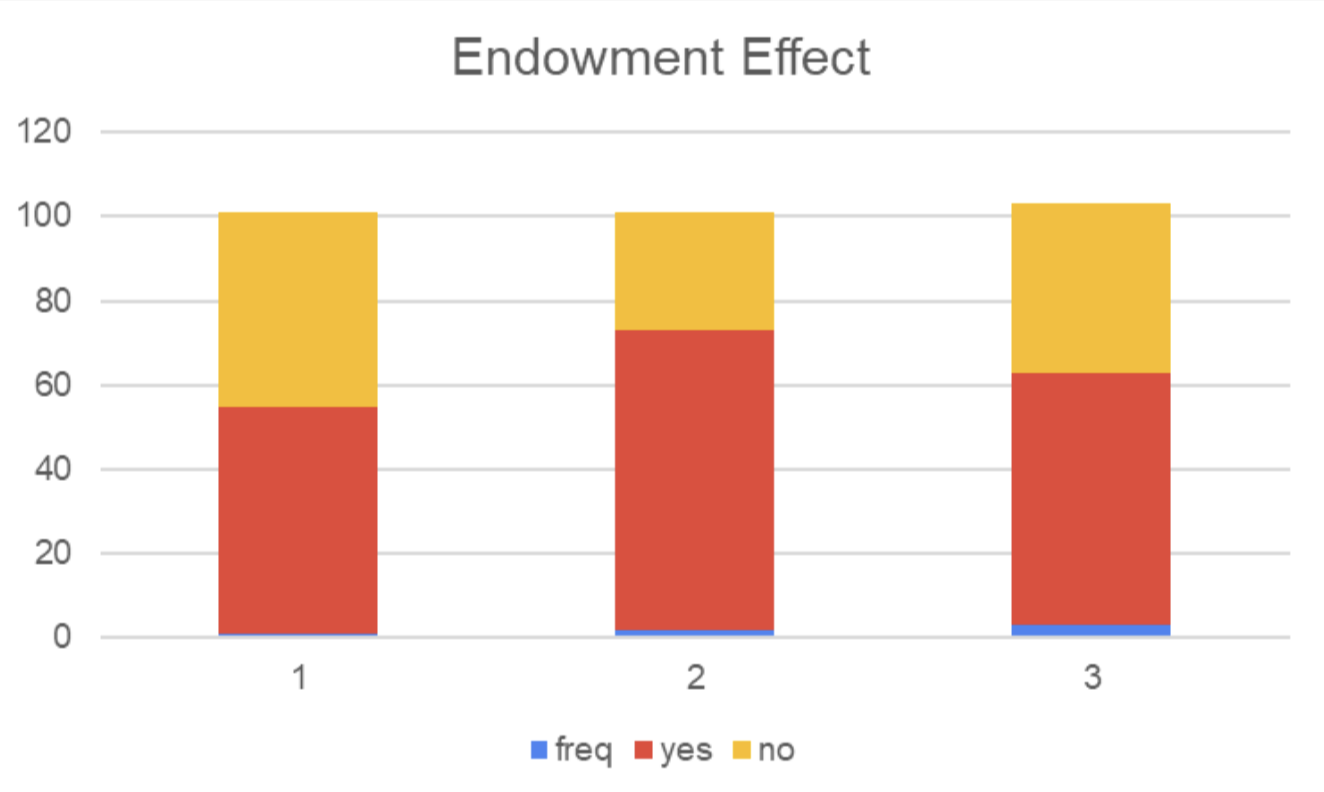
\includegraphics[width=0.5\textwidth]{Endowment.png}}
\caption{Distribution of responses to questions based on endowment and mere exposure effect.}
\label{sr}
\end{figure}

\textbf{Observations:} After aggregating the results from the survey, a stacked bar graph is generated representing the results of all the questions on the same scale. The results show that people are unbiased toward the frequent advertisement, or emails. 54.3\% responded that they do  get affected by frequent postings and the rest said that they do not. While digging deeper to know the attraction, we got to know that the users are more attracted towards the game’s character and their appearance. About 71\% of the respondents got engaged due to this while 28\% did not get affected by the graphics of the characters. Not just looking at the character after fetching the results from the follow up question , we got to know that a game task is given more importance than the character. 65\% of users are engaged due to the task of the application and not just the appearance while visual representation is a matter for the rest 34\%.\

\subsection{Endless scrolling/streaming}
\textbf{Objective:} Flow state, in positive psychology, is the mental state in which an individual, becomes fully absorbed while performing an activity. A state of complete immersion in the work. Developer often try to create this psychological flow in the users. They design apps that are immersive, and more engaging. One of the crucial way in which creators try to achieve this endless scrolling/streaming. For instance, in social media, when users scroll in the infinite-scrolling algorithm, he/she will get more similar on content and they often think they will find something more rewarding. In another example of video platforms, we observe there is no automated stop in video activity or similar suggestions. Because of this, users get more and more absorbed, hence making it difficult for them to stop.

In this section, we kept three questions. The first question takes more direct approach to understand the effect of applications. [\textit{Have you ever felt absorbed due to the endless scrolling features of popular social media apps?}] To get in the positive state of the flow, it is pivotal to be completely immersed in the activity. Second question navigates a different approach to absorb the viewers/users. [\textit{Does recommended contents in applications make it difficult for you to stop surfing?}] The final question asks how much impact does the graphics, working or GUI of the application has on the user. [\textit{Does your efficiency for the same task depend on the theme of the game? This means scoring more if it is a soothing background else not.}]


\begin{figure}[htbp]
\centerline{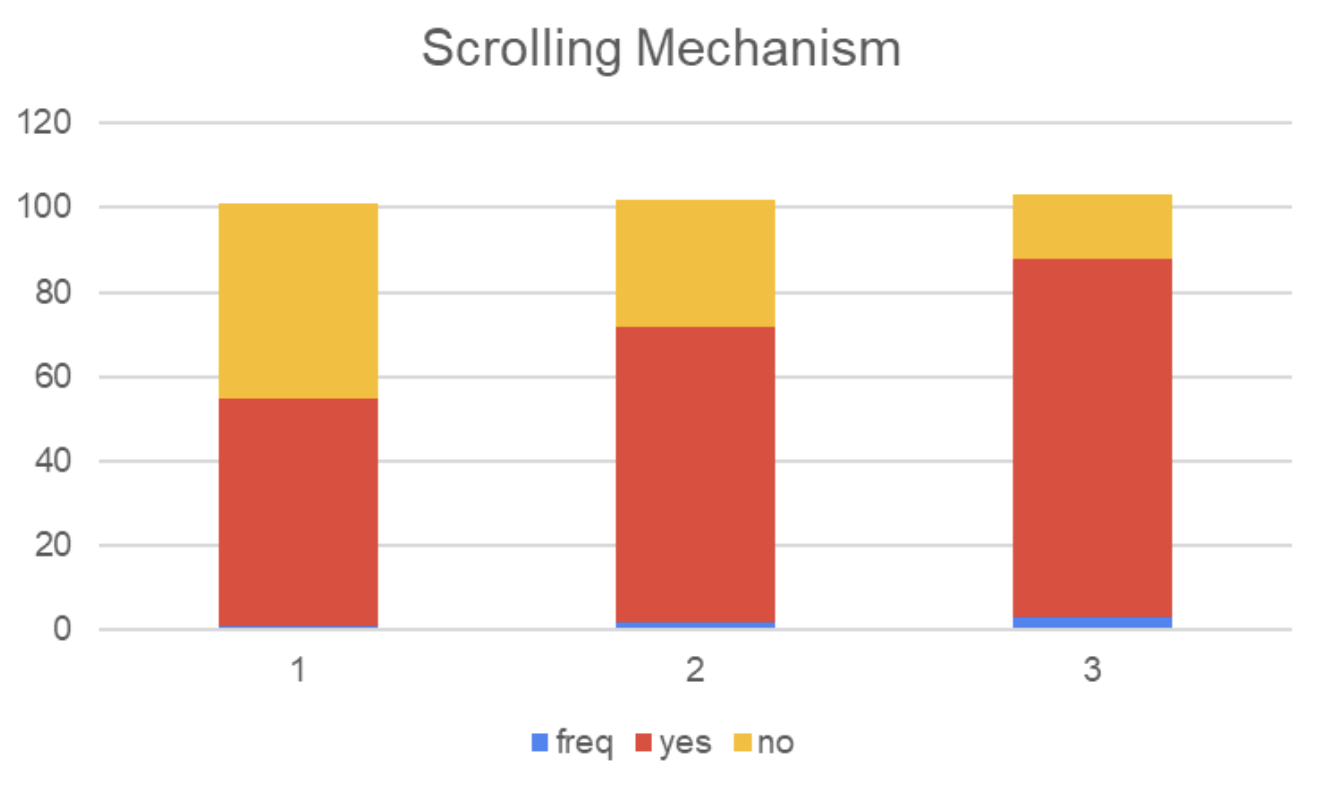
\includegraphics[width=0.5\textwidth]{Endless Scrolling.png}}
\caption{Distribution of responses to questions based on endless scrolling/streaming.}
\label{sr}
\end{figure}

\textbf{Observations: }After aggregating the results from the survey, a stacked bar graph is generated representing the results of all the questions on the same scale. The soothing background of the application keeps more than half of users to use the app while the rest are not affected by it. As the results are close to half, we cannot conclude anything on this research. The direct answer to the question whether endless scrolling keeps you intact with using the application shows that 77\% of users agreed to this notion while others really wanted to use the application. Also the continuous scrolling feature shows recommended posts and slightly more than quarter of respondents were more supportive to this fact  that this keeps them engaged while 32.5\% refused it.

\subsection{Social Pressure}
\textbf{Objective:} Pressure is very monumental aspect to consider when dealing with the inaction. It motives us to take on the work. The same technique can be seen is used by the developers. They try to impose social pressure, the necessity to take part in the activity happening virtually. Sometimes it is observed that users are left with no choice but to participate in the to-and-fro of conservation in the online platform. Moreover, creators also adds the last activity, last seen function in the app, which puts pressure for the user to perform an activity, like reply to a message. 

In this fragment, we have asked the respondents one basic, yet direct and crucial question. [\textit{Do you sometimes feel pressured to interact with someone online just because the other person is aware of your activity [e.g., other person knows you have seen their message]?}] We want to observe whether social pressure leads to the action of the user, or do they feel socially obliged to play their part of the share in the social platform.\


\begin{figure}[htbp]
\centerline{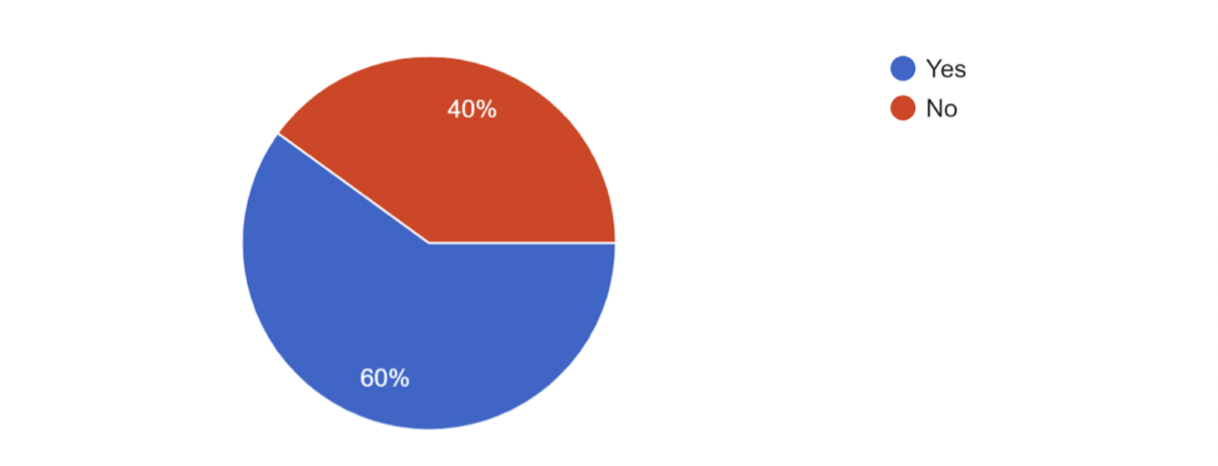
\includegraphics[width=0.5\textwidth]{Social Pressure.png}}
\caption{Distribution of responses to questions based on endowment and mere exposure effect.}
\label{sr}
\end{figure}

\textbf{Observations:} The question was asked to the person who was active on social media. The results from the individual were reported. Converting them to percentages showed that 60\% of the users feel the social thrust of staying on top of the leader-board. The facts and figures related to their post affected them too much. Just like the grades in a school. While the other 40\% refused that they do not feel the pressure of numbers, they just like to interact and be social. The numbers just help them to know the likeness of a post. 

\subsection{Show users of an app what they like}
\textbf{Objective:} An important ingredient to extent the duration of the social media platform is ‘HomePage’ or ‘Newsfeed’. Developers will try to show more and more relevant content to their users. They intend to show the content that is most interesting which wouldn’t get the users bored and they stay attached to the app. Many features such as likes, comment, shares, moreover how long does user hover certain thing are recorded. As a result the algorithm, will provide us with more similar and relevant posts. This is not limited to only posts. Along with it, we also get the advertisement of appropriate and fitting products.

In this section, we have raised few ethical questions, and asked both, users and developers their ethical views. First questions deals with the major ethical question in the field of computer science, selling users data. [\textit{Social media apps collect information about the user so that they can present more targeted content. There’s understandably a tradeoff between ethicality [collecting and selling user data] and practicality [being able to watch favorite shows/content quickly] in this scenario. From a user’s perspective, do you think a user will want to compromise on practicality?}] The follow up of this question os for the developers and understanding their views on the ethically. [\textit{Follow-up: from a developer’s perspective, do you think a user will want to compromise on practicality?}] Third question talks whether user demand for the relevant content. [\textit{Do you believe IT applications should offer suggestions based on user activity logs such that search results or systems’ suggestions could be directed in specific directions?}] Final question from this fragment is asked to the users, [\textit{Would you still use your favorite social media app if they stop tailoring your feed with contents suggested from your past activity on the app or past activities on other apps?}]\

\begin{figure}[htbp]
\centerline{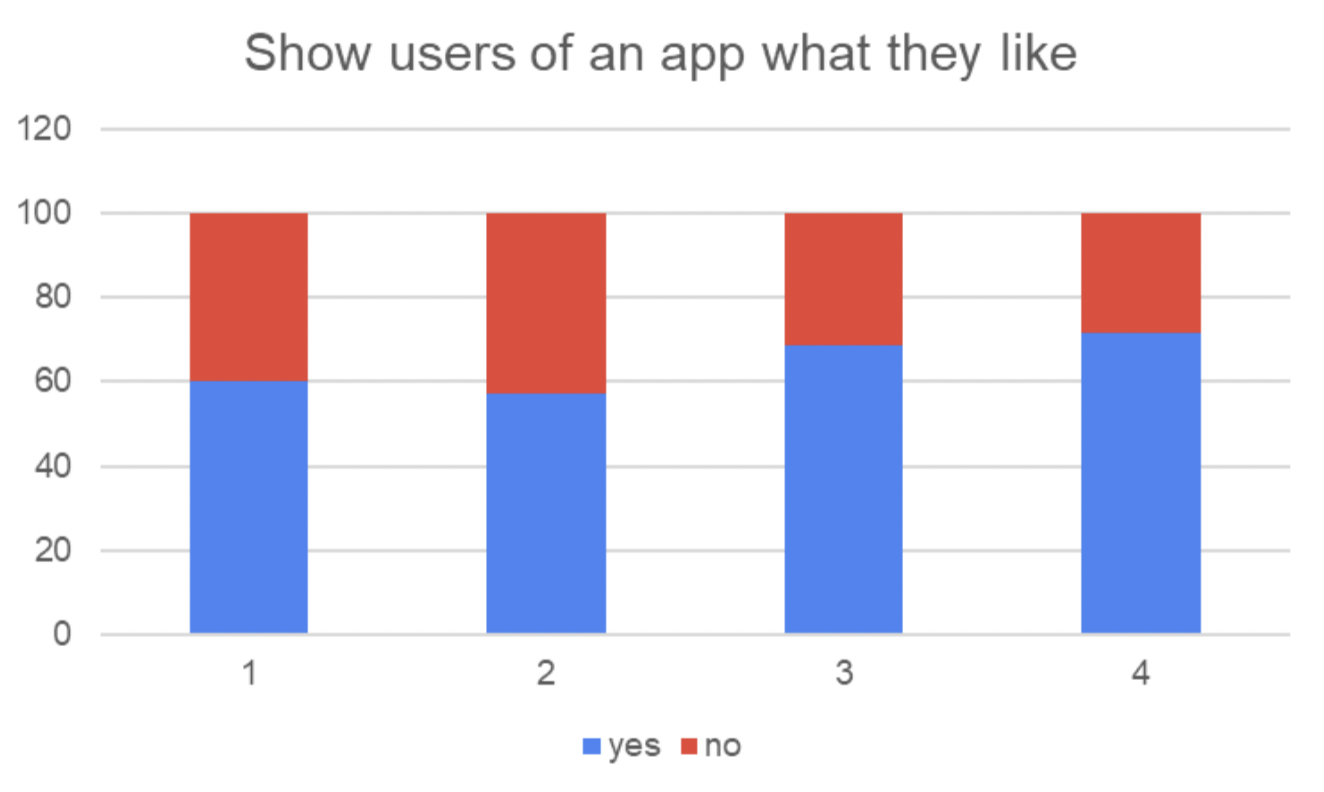
\includegraphics[width=0.5\textwidth]{Showing user relevant posts.png}}
\caption{Distribution of responses to questions based on showing user relevant content.}
\label{sr}
\end{figure}

\textbf{Observations:} 
Based on the observed responses from the users, we plotted the bar graph for the above mention questions. In the fist question, we notice ambiguous thoughts. The question asked was important and deep, 57.1\% of the respondents answered they wanted to compromise the practically but should be able to watch their favourite shows and suggested content. However, we notice a contrast trend from the developers point of view. Majority (68.8\%) are not willing to trade practicality of users for the sake of algorithm. Moreover, from the responses we depict 6 out of every 10 users want the applications to feed them alike posts. However, we can notice the endowment effect in the next question, even if viewers are not offered tailor made content into their feed, almost quarter of them will still use the application. 

\section{Discussion}
Lorem ipsum dolor sit amet, consectetur adipiscing elit, sed do eiusmod tempor incididunt ut labore et dolore magna aliqua. Ut enim ad minim veniam, quis nostrud exercitation ullamco laboris nisi ut aliquip ex ea commodo consequat. Duis aute irure dolor in reprehenderit in voluptate velit esse cillum dolore eu fugiat nulla pariatur. Excepteur sint occaecat cupidatat non proident, sunt in culpa qui officia deserunt mollit anim id est laborum.

\section{Conclusion}
Lorem ipsum dolor sit amet, consectetur adipiscing elit, sed do eiusmod tempor incididunt ut labore et dolore magna aliqua. Ut enim ad minim veniam, quis nostrud exercitation ullamco laboris nisi ut aliquip ex ea commodo consequat. Duis aute irure dolor in reprehenderit in voluptate velit esse cillum dolore eu fugiat nulla pariatur. Excepteur sint occaecat cupidatat non proident, sunt in culpa qui officia deserunt mollit anim id est laborum.

\section{Acknowledgement}
The authors thank Dr. Mohammed Farghally for providing the opportunity to work on such an interesting topic as part of our course project.


\section{IEEE template placeholders}
\subsection{This is a List}
\begin{itemize}
\item Hello
\item There
\item General
\item Kenobi
\end{itemize}

\subsection{Equations}
This is an equation:
\begin{equation}
a+b=\gamma\label{eq}
\end{equation}


\subsection{Figures and Tables}
\paragraph{Positioning Figures and Tables} Place figures and tables at the top and 
bottom of columns. Avoid placing them in the middle of columns. Large 
figures and tables may span across both columns. Figure captions should be 
below the figures; table heads should appear above the tables. Insert 
figures and tables after they are cited in the text. Use the abbreviation 
``Fig.~\ref{fig}'', even at the beginning of a sentence.

\begin{table}[htbp]
\caption{Table Type Styles}
\begin{center}
\begin{tabular}{|c|c|c|c|}
\hline
\textbf{Table}&\multicolumn{3}{|c|}{\textbf{Table Column Head}} \\
\cline{2-4} 
\textbf{Head} & \textbf{\textit{Table column subhead}}& \textbf{\textit{Subhead}}& \textbf{\textit{Subhead}} \\
\hline
copy& More table copy$^{\mathrm{a}}$& &  \\
\hline
\multicolumn{4}{l}{$^{\mathrm{a}}$Sample of a Table footnote.}
\end{tabular}
\label{tab1}
\end{center}
\end{table}

\begin{figure}[htbp]
\centerline{
\includegraphics{fig1.png}}
\caption{Example of a figure caption.}
\label{fig}
\end{figure}


Figure Labels: Use 8 point Times New Roman for Figure labels. Use words 
rather than symbols or abbreviations when writing Figure axis labels to 
avoid confusing the reader. As an example, write the quantity 
``Magnetization'', or ``Magnetization, M'', not just ``M''. If including 
units in the label, present them within parentheses. Do not label axes only 
with units. In the example, write ``Magnetization (A/m)'' or ``Magnetization 
\{A[m(1)]\}'', not just ``A/m''. Do not label axes with a ratio of 
quantities and units. For example, write ``Temperature (K)'', not 
``Temperature/K''.


\begin{thebibliography}{00}

\bibitem{wu2016} Wu, Tim. "The attention merchants: The epic scramble to get inside our heads". Vintage, 2017.
\bibitem{williams2018} Williams, James. "Stand out of our light: freedom and resistance in the attention economy". Cambridge University Press, 2018.
\bibitem{pwc2018} PWC. "IAB Internet Advertising Revenue report". 2018.
\bibitem{campbell2005} Campbell, Marilyn A. "Cyber bullying: An old problem in a new guise?." Journal of Psychologists and Counsellors in Schools, 2005
\bibitem{huey2015} Huey, Laura. "This is Not Your Mother's Terrorism: Social Media, Online Radicalization and the Practice of Political Jamming.". Journal of Terrorism Research 6.2, 2015.
\bibitem{sunstein2017} Sunstein, Cass. "\# Republic: Divided Democracy in the Age of Social Media", Princeton University Press, Princeton, 2017.
\bibitem{uswitch2021} Hiley, Catherine, "How much of your time is Screen Time?". USwitch, 2021.
\bibitem{th1996} Thompson, Steve. Internet connectivity: addiction and dependency study. Diss. Pennsylvania State University, 1996.
\bibitem{gr1998} Gackenbach, Jayne, "Psychology and the Internet: Intrapersonal, interpersonal, and transpersonal implications". Elsevier, 2011.
\bibitem{sc2018} Scholz, Roland W., et al. "Unintended side effects of the digital transition: European scientists’ messages from a proposition-based expert round table". Sustainability, 2018.
\bibitem{duke2017} Duke, Éilish, and Christian Montag. "Smartphone addiction and beyond: Initial insights on an emerging research topic and its relationship to Internet addiction". Internet addiction. Springer, Cham, 2017.
\bibitem{twenge2018} Twenge J.M., Martin G.N., Campbell W.K. "Decreases in psychological well-being among American adolescents after 2012 and links to screen time during the rise of smartphone technology". Emotion. 2018.
\bibitem{ward2017} Ward A.F., Duke K., Gneezy A., Bos M.W. "Brain drain: The mere presence of one’s own smartphone reduces available cognitive capacity". J. Assoc. Consum. Res. 2017.
\bibitem{pontes19} Pontes H.M., Schivinski B., Sindermann C., Li M., Becker B., Zhou M., Montag C. "Measurement and conceptualization of Gaming Disorder according to the World Health Organization framework: The development of the Gaming Disorder Test". International Journal of Mental Health and Addiction, 2019.
\bibitem{sha2019} Sha P., Sariyska R., Riedl R., Lachmann B., Montag C. "Linking Internet Communication and Smartphone Use Disorder by Taking a Closer Look at the Facebook and WhatsApp Applications". Addictive Behaviors Reports, 2019
\bibitem{alter2017} Alter A. "Irresistible: The Rise of Addictive Technology and the Business of Keeping Us Hooked". Penguin Press, 2017.
\bibitem{king11} King D.L., Delfabbro P.H., Griffiths M.D. "The Role of Structural Characteristics in Problematic Video Game Play: An Empirical Study". International Journal of Mental Health and Addiction, 2011.
\bibitem{alu18} Alutaybi A., Mcalaney J., Stefanidis A., Phalp K., McAlaney J., Ali R. "Designing Social Networks to Combat Fear of Missing Out". Proc. Br. HCI, 2018.
\bibitem{gr2018} Griffiths, Mark D. "Adolescent social networking: How do social media operators facilitate habitual use?". Education and Health, 2018.
\bibitem{bosker2016} Bianca B. "THE BINGE BREAKER". Atlantic, 2016.
\bibitem{harris2019} Harris, Tristan. "Optimizing for engagement: Understanding the use of persuasive technology on internet platforms". US Senate Testimony on behalf of Center for Humane Technology, 2019.
\bibitem{morgan2017} Morgans, Julian. "Your addiction to social media is no accident". Vice Media, 2017.
\bibitem{zie1927} Zeĭgarnik B.V. "Über das Behalten von Erledigten und Unerledigten Handlungen". J. Springer, 1927.
\bibitem{kina1928} Rickers-Ovsiankina M.A. "Die Wiederaufnahme Unterbrochener Handlungen". Springer, 1928.

\end{thebibliography}

\end{document}
